% !TeX root = ..//diffgeo_main.tex
\chapter{Differenzierbare Mannigfaltigkeiten}
\section*{Worum geht es in der Differentialgeometrie?}
In den ersten Semestern des Mathematikstudiums wird Analysis in linearen Vektorräumen und  metrischen Räumen betrieben. 
Zudem wurden eventuell Banachräume und Hilberträume betrachtet.
Zentrale Objekte dieser Vorlseung sind sogenannte \textbf{Riemannsche Mannigfaltigkeiten} (diese werden in Abschnitt \ref{chapter:riemannschemannigfaltigkeiten}  eingeführt).
Dies sind differenzierbare Mannigfaltigkeiten ausgestattet mit einer Riemannschen Metrik, d.h. einem Objekt, 
welches es uns erlaubt alle wichtigen geometrischen Größen zu beschreiben, wie zum Beispiel Winkel, Längen, etc.
Riemannsche Mannigfaltigkeiten oder allgemeiner differenzierbare Mannigfaltigkeiten sind im Allgemeinen weder lineare Vektorräume noch metrische Räume.
Der fortgeschrittene Leser könnte nun einwenden, dass wir Riemannsche Mannigfaltigkeiten mit der Struktur eines metrischen Raumes ausstatten können. 
Dies stimmt, aber das wissen wir jetzt noch nicht! 
A priori sind Riemannsche Mannigfaltigkeiten keine metrischen Räume. 
Mehr dazu in Abschnitt \ref{chapter:riemannschemannigfaltigkeiten}
. \\
Unser Ziel ist es die Konzepte der Analysis und Geometrie auf diese differenzierbaren Mannigfaltigkeiten zu übertragen.
Somit bleibt die Frage: was sind überhaupt differenzierbare Mannigfaltigkeiten?
Dies ist Gegenstand dieses Kapitels.\\
Wir beginnen zunächst einmal mit einer kurzen Gegenüberstellung der bereits bekannten Konzepte aus dem $\mathbb{R}^n$ mit den korrespondierenden Begriffen der Differentialgeometrie, welche wir in den kommenden Vorlesungen noch genauer kennenlernen werden. \\
Differenzierbare Mannigfaltigkeiten sind topologische Mannigfaltigkeiten mit einer zusätzlichen Struktur, welche uns erlaubt Analysis auf der Mannigfaltigkeit zu betreiben ("wir wollen differenzieren können").\\
Um diesen Satz mit Sinn zu füllen, müssen wir folgende Fragen klären:
\begin{itemize}
\label{item:frage1}
\item[a)]  Was sind topologische Mannigfaltigkeiten?
\label{item:frage2}
\item[b)]  Was ist mit zusätzlicher Struktur gemeint?
\end{itemize} \newpage

Eine kurze Gegenüberstellung einiger Konzepte der Differentialgeometrie mit bereits bekannten Konzepten aus der Mathematik im $\R^n$ soll als kurze Einführung und Motivation für das Studium der Differentialgeometrie dienen.
\begin{figure}[H]
%Vergleich
\begin{figure}[H]
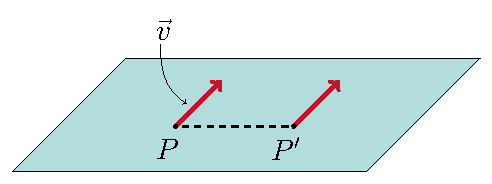
\includegraphics[scale=0.8]{figures/tikz/plane.pdf}
\hspace{2cm}
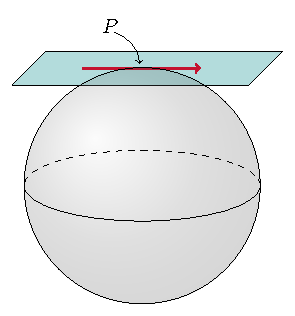
\includegraphics[scale=0.9]{figures/tikz/sphere_with_plane.pdf}
\end{figure}
\centering
\begin{tabular}{>{\centering}p{.45\textwidth} | >{\centering}p{.45\textwidth}} 
$\mathbb{R}^n$ \vspace{5pt} & $\Huge\mathcal{M}$  \vspace{5pt} \tabularnewline \hline 
\vspace{5pt} Parallelverschiebung & \vspace{5pt} Begriff des Zusammenhangs\tabularnewline 
\vspace{5pt} Gerade = kürzeste Verbindung & \vspace{5pt} Konzept der Geodätischen \tabularnewline 
\vspace{5pt} flacher Raum & \vspace{5pt} gekrümmter Raum \tabularnewline 
\vspace{5pt} Skalarprodukt & \vspace{5pt} Riemannsche Metrik \tabularnewline 
\end{tabular}
\end{figure} 

\section{Definitionen}
Wir beginnen damit \hyperref[item:frage1]{a)} zu erläutern.
Topologische Mannigfaltigkeiten sind die zentralen Objekte der Topologie, welches jenes Teilgebiet der Mathematik ist, welches die Eigenschaften von topologischen Räumen untersucht.

Um topologische Mannigfaltigkeiten definieren zu können wiederholen wir zunächst die Definition eines topologischen Raumes. \\
Ein topologischer Raum ist eine Menge $X$ ausgestattet mit einer Topologie, d.h. einer Teilmenge der Potenzmenge von $X$, welche meherern Axiomen genügt.
Topologien erlauben es die zunächst intuitive Anschauung von beispielsweise "Nähe" mathematisch zu präzisieren und auf allgemeine Situationen zu übertragen.
Dies ist der allgemeinste Begriff eines Raumes, indem man Konzepte wie Steigkeit, Konvergenz, Kompaktheit und Zusammenhang sinnvoll definieren kann. 
Metrische Räume sind z.B. topologische Räume mit mehr Struktur.
\phantom{.}\\
\textbf{Erinnerung}: $M \subseteq \mathbb{R}^n$ offen, wenn $\forall p \in U \ \exists \ \varepsilon>0$, sodass $B_{\varepsilon}(p) \subset U$. Dieser Begriff von Offenheit heißt \textit{euklidische Topologie} und erfüllt:
\begin{enumerate}
\item[i)] $\emptyset, \mathbb{R}^n$ offen
\item[ii)] $U, V \subset \mathbb{R}^n$ offen $\Rightarrow U \cap V$ offen in $\mathbb{R}^n$
\item [iii)] $U_i, i \in $ I offen in $\mathbb{R}^n \Rightarrow \bigcup\limits_{i \in \text{I}} U_i \subset \mathbb{R}^n$ offen
\end{enumerate} 

\begin{figure}[H]
\centering
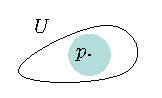
\includegraphics[scale=1.5]{figures/tikz/openset.pdf}
\caption{Offene Menge}
\label{img:offenemenge}
\end{figure} 

\begin{defs}[Topologischer Raum]
Ein topologischer Raum ist eine Menge $X$ zusammen mit einer Menge $\mathcal{T} \subset \mathcal{P}(X)$, sodass:
\begin{enumerate}
\item[i)] $\emptyset, X \in \mathcal{T}$
\item[ii)] $U, V \in \mathcal{T} \Rightarrow  U \cap V \in \mathcal{T}$
\item [iii)] $U_i \in \mathcal{T} \Rightarrow\bigcup\limits_{i \in \text{I}} U_i \in \mathcal{T}$
\end{enumerate} 
Elemente aus $\mathcal{T}$ heißen offen. 
Komplemente davon abgeschlossen.
\end{defs}

Ein topologischer Raum besteht also aus den Daten $X$ und $\mathcal{T}$.
Oft wird jedoch nur $X$ angegeben, wenn die Wahl von $\mathcal{T}$ aus dem Kontext ersichtlich ist.
Beachten Sie, dass dies unpräzise ist und zu verwechslungen führen kann-so kann eine Menge $X$ mit ganz unterschiedlichen Topologien ausgesattet sein. 
Insbesondere kann z.B. eine Menge $U\subset X$ bezüglich einer Topologie $\mathcal{T}_1$ auf $X$ offen sein, während dies für eine andere Topologie $\mathcal{T}_2$ auf $X$
nicht der Fall ist.

\begin{bem}
Alternativ ist auch eine Definition über abgeschlossene Mengen und Umgebungen möglich.
\end{bem}

\begin{bsp}
\begin{itemize}
\item[1.] Das Ihnen vermutlich am besten vertraute Beispiel ist das des Euklidischen Raums $\R^n$ ausgestattet mit der euklidischen Metrik
\begin{align*}
d(x,y) = \sqrt{\sum_i^n (x_i - y_i)^2}.
\end{align*}
\item[2.] Metrische Räume\\
\end{itemize}
Es gibt aber auch weniger anschauliche Beispiele:

\begin{itemize}
\item[3.] Diskrete offene Mengen
\item[4.] Indiskrete Topologie
\item[5.] Drei Punkte
\item[6.] Hilbertwürfel
\end{itemize}
\end{bsp}

Zum Schluss wollen wir noch ein paar natürliche Konstruktionen von topologischen Räumen aus gebenen topologischen Räumen diskutieren. 
Diese liefern natürlich große Beispielklassen.:
\begin{bsp}
\begin{enumerate}
\item[i)] Produktopologie
\item[ii)] Quotiententopologie
\item[iii)] Teilraumtopologie. \\
	Sei $N$ eine Teilmenge von $X$. Dann ist auch $(N,\mathcal{T}_1)$ ein topologischer Raum, wobei $\mathcal{T}_1$ wie folgt gegeben ist:\\
	\center{$V \in \mathcal{T}_1 \Leftrightarrow \ \exists \ U \in \mathcal{T}$, sodass $V= N \cap U$}
\end{enumerate}
\end{bsp}

\begin{defs}[Topologische Mannigfaltigkeiten]
Eine topologische Mannigfaltigkeit ist ein topologischer Raum $\mathcal{M}$ der Dimension $n$ mit folgenden Eigenschaften:
\begin{enumerate}
	\item[i)] $\mathcal{M}$ ist hausdorffsch. Das heißt für alle $p, q \in \mathcal{M}$ mit $p \neq q $ existieren zwei disjunkte, offene Umgebungen $U \ni p$ und $V \ni q$ wobei $U, V \in \mathcal{T}$
\begin{figure}[H]
\centering
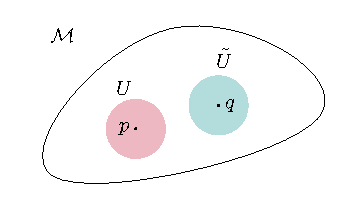
\includegraphics[width=0.4\linewidth]{figures/tikz/hausdorff.pdf}
\caption{Hausdorff'sche Eigenschaft}
\label{img:hausdorff}
\end{figure} 	
	\item[ii)] \textbf{2. Abzählbarkeitsaxiom}  \\
	$\mathcal{M}$ hat eine abzählbare Basis der Topologie, das heißt es existiert eine abzählbare Menge $\{U_1, \dots, U_k, \dots\}$ 
	offener Teilmengen oder abzählbar viele offene Mengen $U_1, \dots, U_k, \dots$ mit $U_i \in \mathcal{T}$, 
	sodass $\forall p \in \mathcal{M}$ und alle Umgebungen $U$ von $p$ gibt es ein $k$ sodass $p \in U_k \subseteq U$.
	\item [iii)] $\mathcal{M}$ ist homöomorph zu $\mathbb{R}^n$, das heißt $\forall p \in \mathcal{M}$ existiert eine Umgebung $U$ von $p$ und ein \bfseries Homöomorphismus \normalfont $X: U \rightarrow V \subseteq \mathbb{R}^n$ (offen).
\end{enumerate} 
\end{defs}
\begin{minipage}[H]{.8\textwidth}
\begin{defs}[Karte, Atlas]
	Das Paar $(X, U)$ heißt \textbf{Karte} von $\mathcal{M}$ um $p$. \\
	Eine Menge $\mathcal{A} = \{(x_{\alpha},U_{\alpha})_{\alpha \in \mathcal{A}}\}$ von Karten heißt \textbf{Atlas} von $\mathcal{M}$, falls \\
	\begin{align}
	\bigcup\limits_{\alpha \in \mathcal{A}} U_\alpha = \mathcal{M}
	\end{align}
\end{defs}
\end{minipage}
\hspace{1cm}
\begin{minipage}[H]{.2\textwidth}
\vspace{-0.5cm}
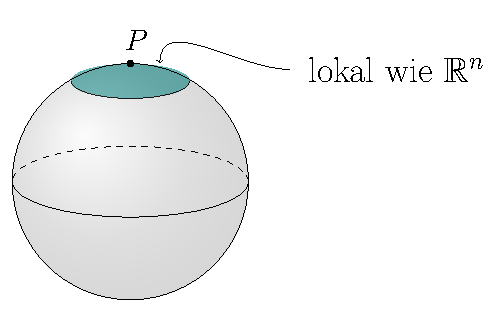
\includegraphics[scale=0.5]{figures/tikz/sphere_local_rn}
\end{minipage}


Topologische Mannigfaltigkeiten sind die Grundbausteine. Nun wollen wir auf diesen Mannigfaltigkeiten Geometrie betreiben. Dafür benötigen wir mehr Struktur. Wir wollen die differenzierbare Struktur des $\mathbb{R}^n$ auf unseren Mannigfaltigkeiten "holen".

\begin{defs}[Kartenwechsel]
Seien $x_{\alpha}$ und $x_{\beta}$ zwei Karten, dann ist der Kartenwechsel wie folgt definiert: \\
\begin{align}
x_{\alpha}\circ x_{\beta}^{-1}: x_{\beta}(U_{\alpha}\cap U_{\beta}) \rightarrow x_{\alpha}(U_{\alpha}\cap U_{\beta}) \subseteq \mathbb{R}^n
\end{align}
Dies ist ein Homöomorphismus.

\begin{figure}[H]
\centering
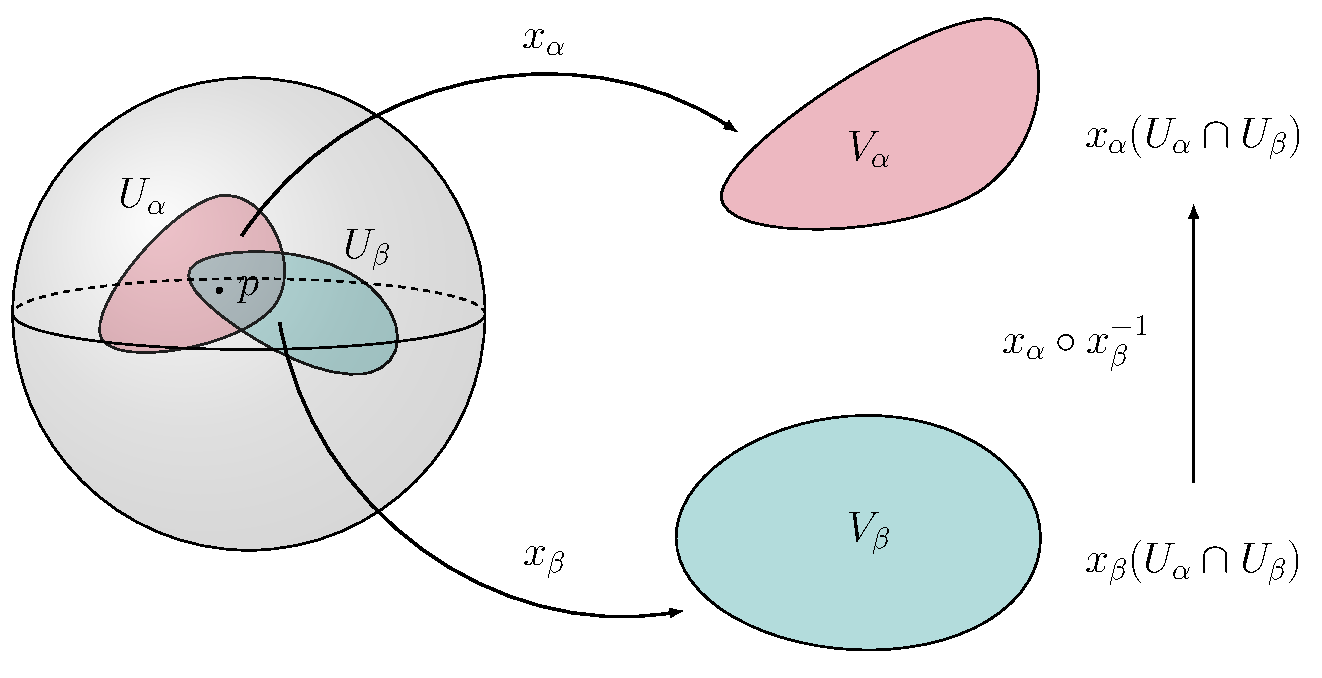
\includegraphics[width=1.0\linewidth]{figures/tikz/map_change.pdf}
\caption{Kartenwechsel}
\label{img:kartenwechsel}
\end{figure} 

\end{defs}
Nun wollen wir, dass $x_{\alpha}\circ x_{\beta}^{-1}$ Diffeomorphismen sind.
\begin{defs}[$C^{\infty}$-Atlas]
Sei $ \mathcal{M}$ eine topologische Mannigfaltigkeit.
\begin{enumerate}
	\item[a)] Ein Atlas $\mathcal{A} = \{(x_{\alpha},U_{\alpha})\}$ auf $\mathcal{M}$ heißt $C^{\infty}$-Atlas, falls alle Kartenwechsel $x_{\alpha}\circ x_{\beta}^{-1}$ mit $\alpha, \beta \in A \ C^{\infty}$-Diffeomorphismen sind.
	\item[b)] Sei $\mathcal{A}$ ein $C^{\infty}$-Atlas von $\mathcal{M}$. \\
	Eine Karte $(x,U)$ ist verträglich mit $\mathcal{A}$, falls $x \circ x_\alpha^{-1}$ ein $C^{\infty}$-Diffeomorphismus ist.
\end{enumerate}
\end{defs}
Gegeben ein $C^{\infty}$-Atlas, so kann man diesen zu einem \textit{maximalen} $C^{\infty}$-Atlas vervollständigen. Maximal bedeutet hierbei, dass der Atlas nicht strikt in einem anderen enthalten ist.

